\section{DFT and the machinery of frequency}

Throughout, $f(x,y)$ is indexed with $x$ the row and $y$ the column of an
$M\times N$ array, and the unnormalised DFT is
\begin{equation}
F(u,v)=\sum_{x=0}^{M-1}\sum_{y=0}^{N-1} f(x,y)\,e^{-j2\pi(ux/M+vy/N)},
\qquad
f(x,y)=\frac{1}{MN}\sum_{u,v}F(u,v)\,e^{+j2\pi(ux/M+vy/N)},
\label{eq:dft}
\end{equation}
which is the convention of \code{numpy.fft.fft2}. Indices are taken modulo $M$
and $N$, so $F(-u,-v)$ means $F(M-u,N-v)$.

\subsection{Build and validate the DFT}

The 1-D DFT matrix is $W_N[u,x]=e^{-j2\pi ux/N}$. Because the kernel in
\eqref{eq:dft} factors as $e^{-j2\pi ux/M}e^{-j2\pi vy/N}$, the double sum is a
sum over $x$ of a sum over $y$:
$F(u,v)=\sum_x W_M[u,x]\sum_y f(x,y)W_N[v,y]=(W_M f W_N^{T})[u,v]$.
\code{dft\_matrix} builds $W_N$ from the integer product $ux \bmod N$ before the
exponential, so the argument of $e^{-j2\pi k/N}$ stays in $[0,2\pi)$ and no
precision is lost to large phases. \code{dft2} is two matrix products, and
\code{idft2} uses $W_N^{-1}=\overline{W_N}/N$.

\begin{table}[H]
\centering
\begin{tabular}{lrrrrrr}
\toprule
Input & $\max|F_c-F_n|$ & $\max|F_n|$ & relative & round trip & custom (s) & \code{fft2} (s)\\
\midrule
\code{q1.png} $512\times512$ & $8.153\times10^{-9}$ & $3.383\times10^{7}$ & $2.41\times10^{-16}$ & $6.452\times10^{-12}$ & 0.0131 & 0.00203\\
\code{q1} crop $256\times384$ & $4.564\times10^{-9}$ & $1.375\times10^{7}$ & $3.32\times10^{-16}$ & $9.265\times10^{-12}$ & 0.0044 & 0.00060\\
normal noise $64\times48$ & $1.208\times10^{-13}$ & $1.464\times10^{2}$ & $8.25\times10^{-16}$ & $3.109\times10^{-15}$ & 0.0001 & 0.00002\\
\bottomrule
\end{tabular}
\caption{Custom separable DFT ($F_c$) against \code{numpy.fft.fft2} ($F_n$),
complex128; ``round trip'' is $\max|\text{idft2}(F_c)-f|$. The
non-square crop checks that $W_M$ and $W_N$ are used on the correct sides. Times
are medians.}
\label{tab:dft-error}
\end{table}

The largest absolute error on the test image is $8.2\times10^{-9}$, but the
spectrum itself reaches $3.4\times10^{7}$ (the DC term), so the relative error is
$2.4\times10^{-16}$, about one unit of float64 round-off. The matrix version costs
$O(MN(M+N))$ operations against $O(MN\log MN)$ for the FFT, which shows in the
6.5$\times$ time gap at $512\times512$.

\paragraph{(a) Conjugate symmetry.} For real $f$, conjugating \eqref{eq:dft}
only flips the sign of the exponent:
\begin{equation}
\overline{F(u,v)}=\sum_{x,y} f(x,y)\,e^{+j2\pi(ux/M+vy/N)}
=\sum_{x,y} f(x,y)\,e^{-j2\pi((-u)x/M+(-v)y/N)}=F(-u,-v).
\end{equation}
So $|F|$ is even and the phase is odd. Half of the spectrum is redundant: in the
centred display, the half-plane $u<0$ is the point reflection of $u>0$ through the
origin, and on the line $u=0$ the values with $v<0$ mirror those with $v>0$. With
$M,N$ even, the four bins $(0,0)$, $(0,N/2)$, $(M/2,0)$ and $(M/2,N/2)$ are their
own mirror images and must be real. Counting real degrees of freedom gives
$2\cdot\frac{MN-4}{2}+4=MN$, exactly the number of pixels, which is why
\code{rfft2} can store only $M(N/2+1)$ values. On the test image
$\max|F(u,v)-\overline{F(-u,-v)}|=4.146\times10^{-9}$ and the largest imaginary
part at the four self-conjugate bins is $2.073\times10^{-9}$, both round-off.
Viewers still show the whole symmetric spectrum (Fig.~\ref{fig:conj}) because
orientation is easier to read when a line of energy passes through the centre in
both directions, the grid matches the full image so filters can be drawn on it
directly, and the redundant half costs nothing to display.

\begin{figure}[H]
\centering
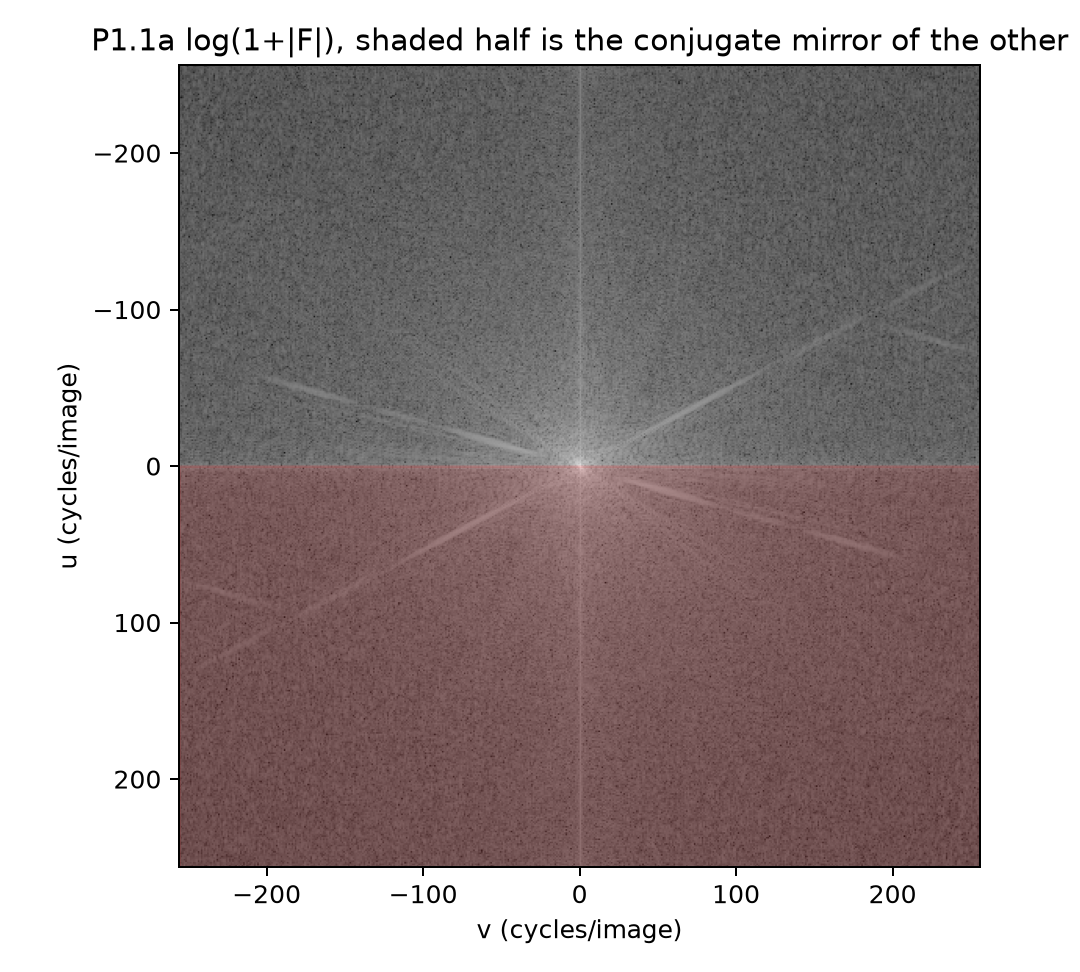
\includegraphics[width=0.45\linewidth]{problem_1/conjugate_symmetry.png}
\caption{Centred $\log(1+|F|)$ of \code{q1.png}. The shaded half is the
conjugate mirror of the other half.}
\label{fig:conj}
\end{figure}

\paragraph{(b) Shift and convolution theorems.} Substituting $x'=x-x_0$ in
\eqref{eq:dft} for a circular shift gives
$f(x-x_0,y-y_0)\leftrightarrow F(u,v)e^{-j2\pi(ux_0/M+vy_0/N)}$: the magnitude is
unchanged and the phase gains a linear ramp. Table~\ref{tab:shift} compares the
custom DFT of shifted copies of the test image (\code{np.roll}) with the
prediction, and lists the measured phase change at a few frequencies.

\begin{table}[H]
\centering
\begin{tabular}{lrrr}
\toprule
$(x_0,y_0)$ & $\max|F_s-F\cdot\text{ramp}|$ & relative & $\max\big||F_s|-|F|\big|$\\
\midrule
$(5,0)$ & $8.330\times10^{-9}$ & $2.46\times10^{-16}$ & $8.382\times10^{-9}$\\
$(0,17)$ & $1.542\times10^{-8}$ & $4.56\times10^{-16}$ & $5.588\times10^{-9}$\\
$(31,-12)$ & $1.201\times10^{-7}$ & $3.55\times10^{-15}$ & $7.451\times10^{-9}$\\
$(200,300)$ & $1.557\times10^{-6}$ & $4.60\times10^{-14}$ & $6.054\times10^{-9}$\\
\midrule
\multicolumn{4}{l}{phase change $\angle(F_s/F)$ in rad, shift $(31,-12)$ and $(200,300)$}\\
\midrule
$(u,v)$ & predicted & measured & $|$difference$|$\\
\midrule
$(1,0)$, shift $(31,-12)$ & $-0.380427$ & $-0.380427$ & $4.44\times10^{-16}$\\
$(50,-20)$, shift $(31,-12)$ & $-3.117049$ & $-3.117049$ & $3.55\times10^{-15}$\\
$(-100,140)$, shift $(31,-12)$ & $2.110758$ & $2.110758$ & $7.55\times10^{-15}$\\
$(0,1)$, shift $(200,300)$ & $2.601631$ & $2.601631$ & $8.88\times10^{-16}$\\
$(50,-20)$, shift $(200,300)$ & $1.178097$ & $1.178097$ & $5.33\times10^{-15}$\\
$(-100,140)$, shift $(200,300)$ & $0.196350$ & $0.196350$ & $1.87\times10^{-14}$\\
\bottomrule
\end{tabular}
\caption{2-D shift theorem on \code{q1.png} with the custom DFT. The full list of
20 phase checks is in \code{results/problem\_1/shift\_theorem\_table.txt}.}
\label{tab:shift}
\end{table}

The error grows with the shift because the ramp phase $2\pi(ux_0/M+vy_0/N)$ reaches
larger values before it is wrapped, so its round-off grows with it, but even at
$(200,300)$ the relative error is $4.6\times10^{-14}$.

For circular convolution
$g(x,y)=\sum_{m,n}h(m,n)f(x-m,y-n)$ with indices mod $M,N$, substituting into
\eqref{eq:dft} and swapping the sums gives $G=F\cdot H$, where $H$ is the DFT of the
kernel placed on the image grid with its origin at index $(0,0)$. The spatial side
was computed directly, one \code{np.roll} per kernel tap, and the frequency side as
$\text{idft2}(\text{dft2}(f)\,\text{dft2}(h))$ with the custom transforms.

\begin{table}[H]
\centering
\begin{tabular}{lrrrrr}
\toprule
Kernel & $\max|g_s-g_f|$ & $\max|g_s|$ & relative & $\max|\operatorname{Im} g_f|$ & $\max|G_s-FH|$\\
\midrule
box $3\times3$ & $2.501\times10^{-12}$ & $2.550\times10^{2}$ & $9.81\times10^{-15}$ & $3.145\times10^{-13}$ & $1.398\times10^{-8}$\\
Laplacian $5\times5$ & $6.412\times10^{-11}$ & $1.851\times10^{3}$ & $3.46\times10^{-14}$ & $5.699\times10^{-12}$ & $3.317\times10^{-8}$\\
random $7\times7$ & $4.093\times10^{-11}$ & $4.463\times10^{3}$ & $9.17\times10^{-15}$ & $4.736\times10^{-12}$ & $3.255\times10^{-7}$\\
\midrule
$(u,v)$, random kernel & \multicolumn{2}{r}{predicted $F H$} & \multicolumn{3}{r}{measured DFT of $f\circledast h$}\\
\midrule
$(0,0)$ & \multicolumn{2}{r}{$-5.627403\times10^{8}$} & \multicolumn{3}{r}{$-5.627403\times10^{8}$}\\
$(5,3)$ & \multicolumn{2}{r}{$6.338837\times10^{6}-8.990184\times10^{6}j$} & \multicolumn{3}{r}{$6.338837\times10^{6}-8.990184\times10^{6}j$}\\
$(100,-40)$ & \multicolumn{2}{r}{$-6.964199\times10^{3}-4.627895\times10^{3}j$} & \multicolumn{3}{r}{$-6.964199\times10^{3}-4.627895\times10^{3}j$}\\
$(-200,17)$ & \multicolumn{2}{r}{$-5.036941\times10^{3}+9.049523\times10^{3}j$} & \multicolumn{3}{r}{$-5.036941\times10^{3}+9.049523\times10^{3}j$}\\
\bottomrule
\end{tabular}
\caption{2-D circular convolution theorem on \code{q1.png}; $g_s$ is the direct
spatial result, $g_f$ the frequency-domain one and $G_s$ the DFT of $g_s$. The random kernel is
asymmetric (seed 7), so a flipped kernel or a misplaced origin would show up as a
large error.}
\label{tab:conv}
\end{table}

\paragraph{(c) Sinusoid parameter recovery.} The synthetic $256\times256$ image is
$f(x,y)=128+\sum_i A_i\cos(2\pi(u_ix+v_iy)/N+\phi_i)$ with the ground truth of
Table~\ref{tab:sin}. Writing each cosine as two complex exponentials shows that it
contributes $\tfrac{A_i}{2}MN\,e^{\pm j\phi_i}$ at $\pm(u_i,v_i)$ and nothing
elsewhere when $u_i,v_i$ are integers. The recovery therefore reads every peak
above $10^{-3}$ of the largest non-DC peak, keeps the member of each conjugate pair
with $u>0$ (or $u=0,v>0$), and returns $A=2|F|/MN$ and $\phi=\angle F$; the offset
is $F(0,0)/MN$. Only the spectrum is used, not the ground truth.

\begin{table}[H]
\centering
\begin{tabular}{lrrrrrr}
\toprule
$(u_i,v_i)$ cycles/image & $A$ true & $A$ found & $|\Delta A|$ & $\phi$ true & $\phi$ found & $|\Delta\phi|$\\
\midrule
$(6,10)$ & 50.00 & 50.0000000000 & $1.4\times10^{-14}$ & 0.785398 & 0.785398 & $3.6\times10^{-15}$\\
$(20,-14)$ & 30.00 & 30.0000000000 & $3.6\times10^{-15}$ & $-1.047198$ & $-1.047198$ & $1.3\times10^{-15}$\\
$(0,45)$ & 20.00 & 20.0000000000 & 0 & 2.000000 & 2.000000 & $4.4\times10^{-15}$\\
$(90,5)$ & 10.00 & 10.0000000000 & $3.6\times10^{-15}$ & $-2.500000$ & $-2.500000$ & $1.1\times10^{-14}$\\
\bottomrule
\end{tabular}
\caption{Ground truth and recovered parameters. Exactly four peaks were found and
the recovered offset is 128.0000000000.}
\label{tab:sin}
\end{table}

\textbf{Resolution limit.} An $N$-point DFT samples the spectrum of the finite
signal at $u/N$ cycles per pixel, so the grid spacing is
$\Delta f=1/N$ cycles/pixel, i.e.\ one cycle per image ($1/256=0.003906$ here).
The origin is the finite observation window: the $N$ samples are the infinite
signal times a length-$N$ rectangle, so every spectral line is convolved with the
Dirichlet kernel $D_N(\nu)=\sin(\pi N\nu)/(N\sin(\pi\nu))$, whose main lobe is
$2/N$ wide. Two components closer than about $1/N$ merge into one lobe, and no
amount of zero padding separates them, because zero padding only samples the same
blurred spectrum more finely. Fig.~\ref{fig:sin} shows both effects. Two cosines
$0.5$ cycles/image apart give one main peak even in a $16\times$ zero-padded
spectrum, while $1.5$ cycles/image apart they give two. A single cosine at the
off-grid frequency $10.5$ is read as amplitude $31.07$ and $32.56$ from the two
nearest bins against a true 50; the Dirichlet prediction for a half-bin offset is
$50\,|D_N(1/2N)|=31.83$. Its energy also leaks, so 33 bins exceed one grey level.

\begin{figure}[H]
\centering
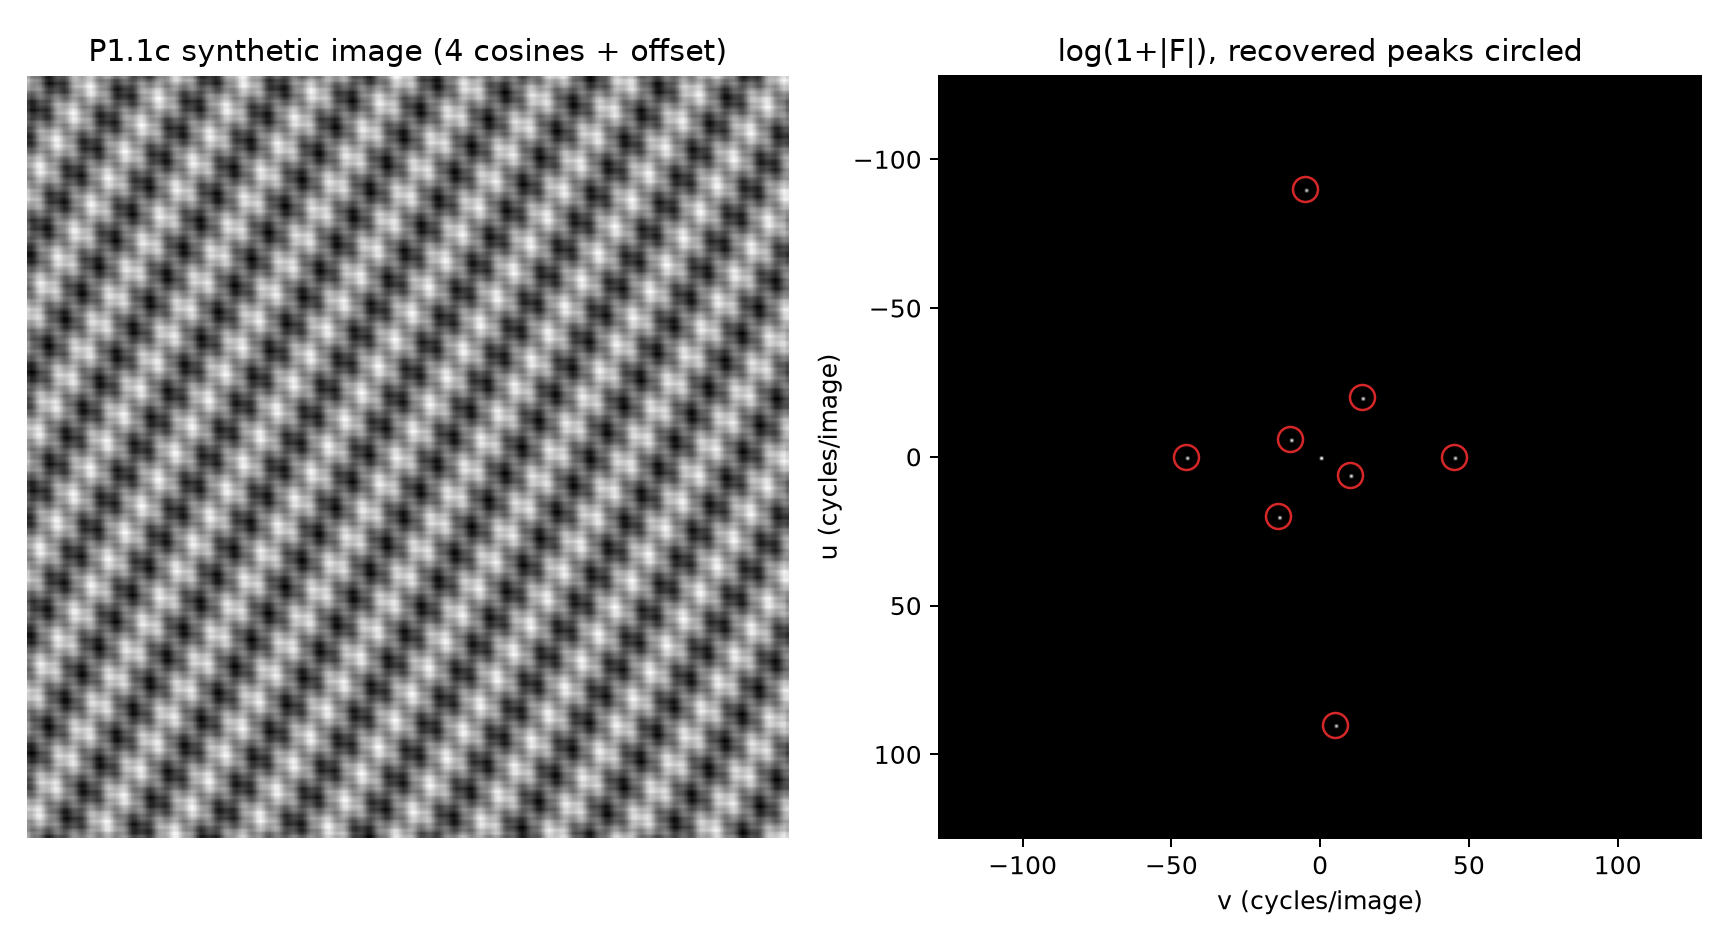
\includegraphics[width=0.72\linewidth]{problem_1/sinusoid_recovery.png}\\
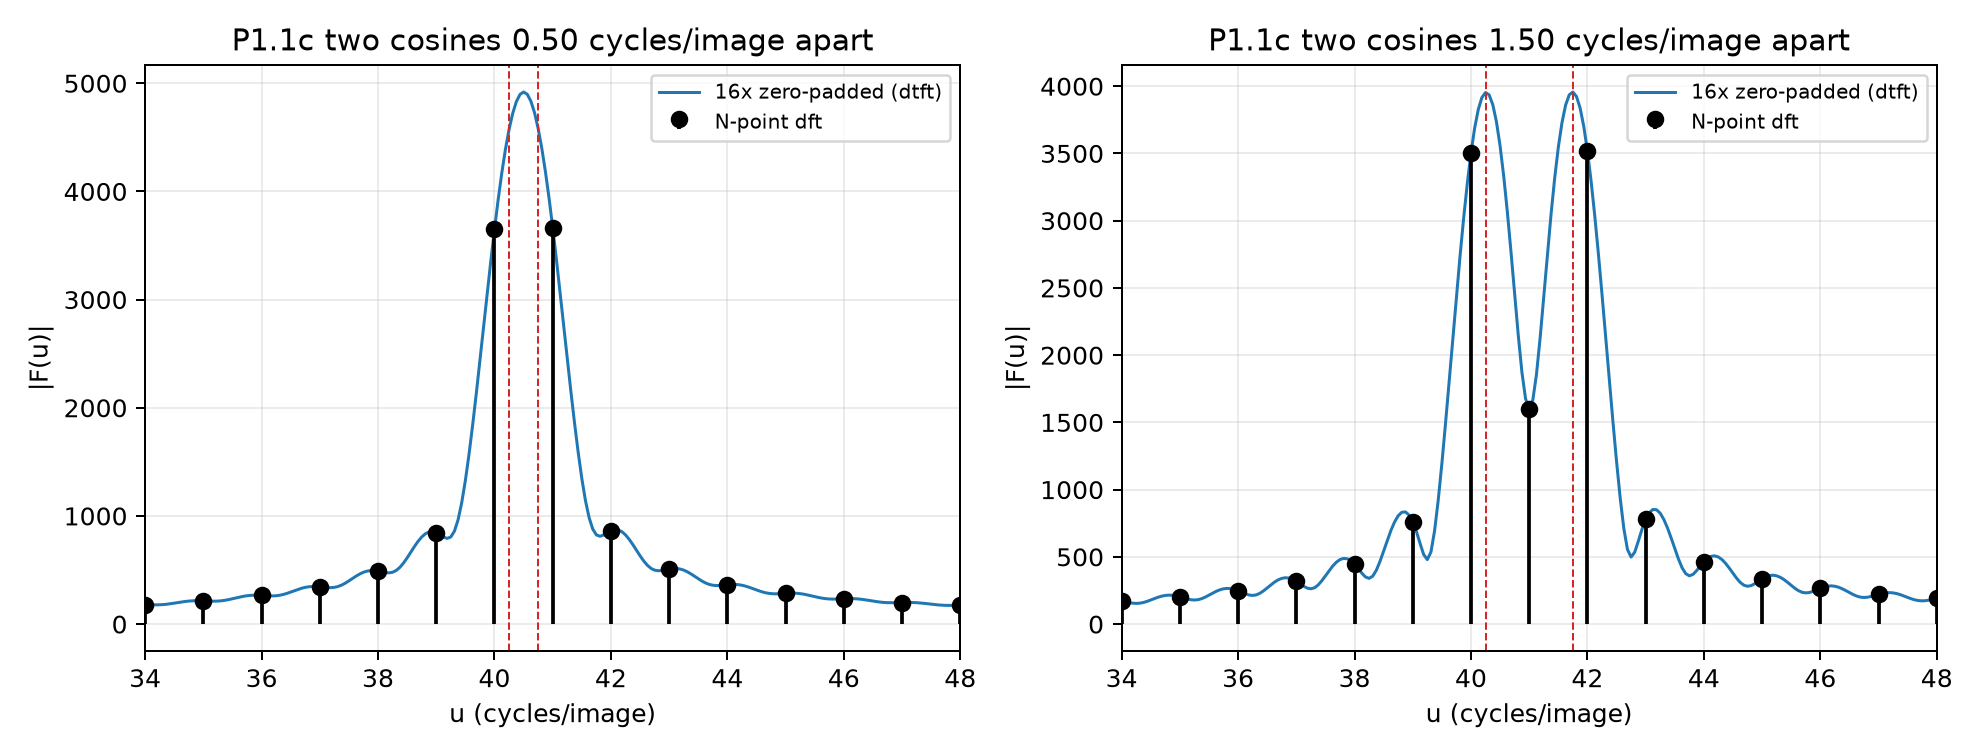
\includegraphics[width=0.85\linewidth]{problem_1/resolution_limit.png}
\caption{Top: synthetic image and its centred log spectrum with the recovered peaks
circled. Bottom: two cosines $0.5$ and $1.5$ cycles/image apart, 256-point DFT
(stems) and $16\times$ zero-padded spectrum (line).}
\label{fig:sin}
\end{figure}

\subsection{Phase versus magnitude}

That phase carries most of the structure of an image is a classical observation
\cite{oppenheim}; this section predicts and measures how much.


\textbf{Prediction.} The analytical prediction is in
\code{docs/predictions/p1\_2\_phase\_magnitude\_prediction.md}, written on
2026-10-23 at 16:28 and committed at 16:29 (commit \code{3c9e956}), seven minutes
before the experiment code was committed (\code{164d182}, 16:36). In short: for
uniform white noise $n$ of the same size, $|N(u,v)|$ is close to Rayleigh
distributed away from DC, so $|N|=\mu(1+\epsilon)$ with
$\operatorname{var}\epsilon=4/\pi-1=0.273$. By superposition
$r=\text{idft}(|N|e^{j\phi})=\mu p+\mu\,\text{idft}(\epsilon e^{j\phi})+\text{const}$,
where $p=\text{idft}(e^{j\phi})$ is the flat-magnitude image. By the shift theorem a
feature at $(x_k,y_k)$ carries the linear phase $e^{-j2\pi(ux_k/M+vy_k/N)}$, and a
linear phase with flat magnitude inverts to an impulse at $(x_k,y_k)$, so $p$ should
concentrate at the positions of edges and lines (equivalently $p=f\circledast
\text{idft}(1/|F|)$, a whitening high-pass). The second term is $p$ convolved with
the white field $\text{idft}(\epsilon)$, a stationary speckle, and Parseval predicts
its energy relative to the first as $\operatorname{E}\epsilon^2=0.273$, so a
least-squares fit $r=cp+\text{residual}$ should leave a residual of 27\,\% of
$\|cp\|^2$ and $\operatorname{corr}(r,p)\approx1/\sqrt{1.273}=0.89$.

\begin{figure}[H]
\centering
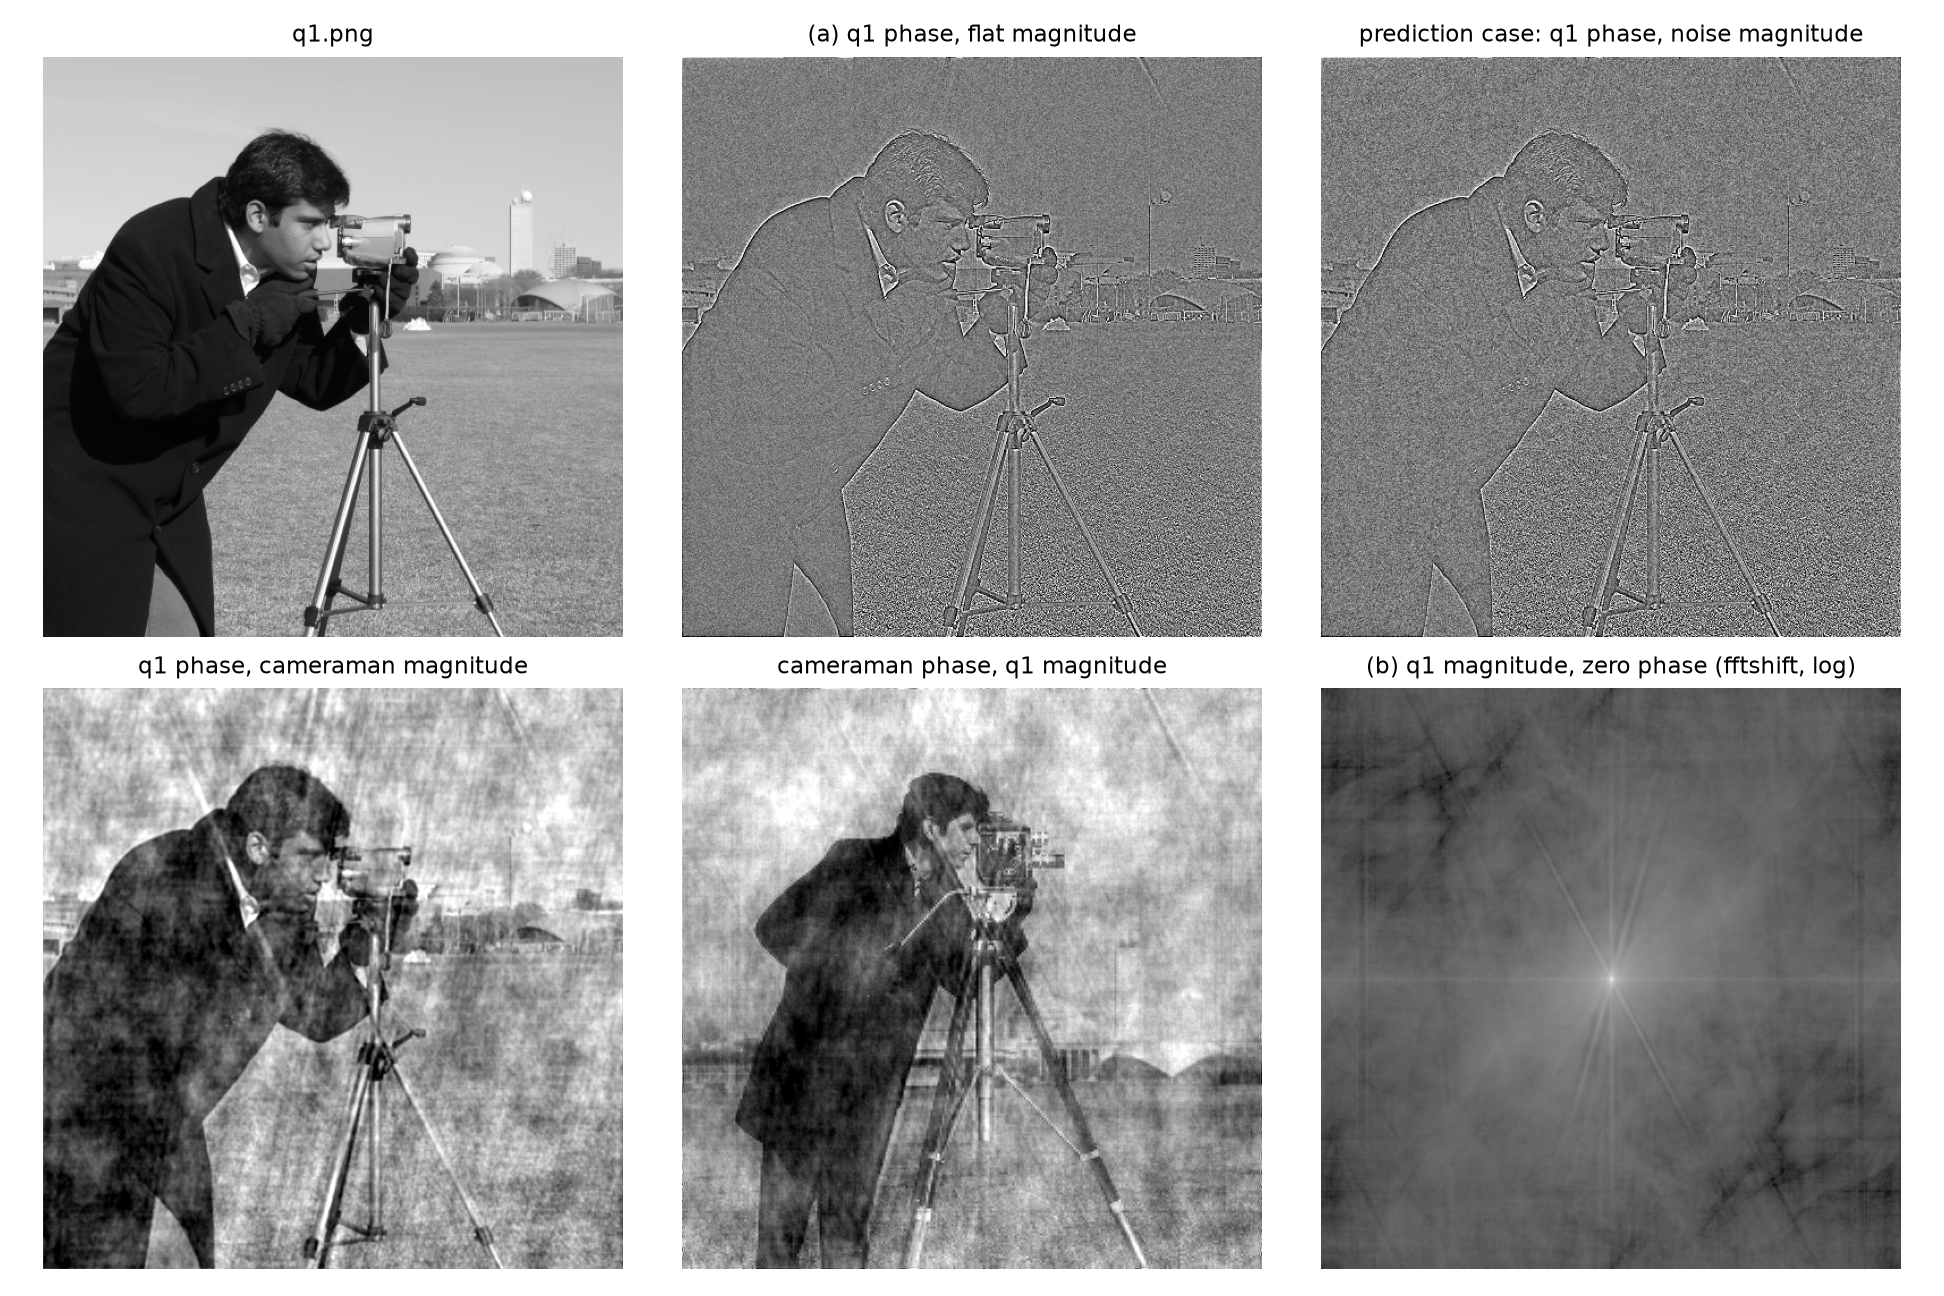
\includegraphics[width=\linewidth]{problem_1/phase_magnitude.png}
\caption{Phase and magnitude experiments on \code{q1.png} (custom transforms).
Each panel is stretched between its 0.5 and 99.5 percentiles; the zero-phase
panel is $\log(1+|r_0|)$ after \code{fftshift}.}
\label{fig:phase}
\end{figure}

\paragraph{(a) Flat magnitude.} The phase-only image (Fig.~\ref{fig:phase}, top
middle) shows the outline of the photographer, the coat edge, the tripod legs and
the buildings at their true positions as thin bright and dark lines, and has no
large-scale shading: $\operatorname{corr}(p,f)=0.18$ while
$\operatorname{corr}(|p|,|\nabla f|)=0.48$. The noise-magnitude case matches the
prediction closely (Table~\ref{tab:phase}). The measured $\operatorname{var}\epsilon$
is 0.2744, the residual-to-structure energy ratio is 0.2744 against the predicted
0.273, and $\operatorname{corr}(r,p)=0.8858$ against 0.89. The two ratios agree to
four digits because, with the same phase, the residual is exactly the
$\epsilon$-weighted part of the spectrum.

\begin{table}[H]
\centering
\begin{tabular}{lrr}
\toprule
Quantity & predicted & measured\\
\midrule
$\operatorname{var}\epsilon$ of the noise magnitude (DC excluded) & $4/\pi-1=0.2732$ & 0.2744\\
energy(residual) / energy($cp$) & 0.273 & 0.2744\\
$\operatorname{corr}(r,p)$ & 0.89 & 0.8858\\
$\operatorname{corr}(|p|,|\nabla f|)$ / $\operatorname{corr}(|r|,|\nabla f|)$ & speckle lowers it & 0.4806 / 0.4077\\
\bottomrule
\end{tabular}
\caption{Prediction against measurement for the noise-magnitude reconstruction
(uniform noise, seed 2026).}
\label{tab:phase}
\end{table}

One part of the prediction did not hold. It said flat areas such as the sky would
go to a uniform grey. They carry a fine grain instead (Fig.~\ref{fig:phase} and
\code{phase\_magnitude\_zoom.png}). The sky in the photograph is not exactly flat:
it has small sensor and compression fluctuations, and dividing by $|F|$ boosts the
high frequencies where those fluctuations live as much as it boosts edges.
Whitening cannot tell a weak high-frequency texture from a strong one.

Flat magnitude isolates phase more cleanly than swapping magnitudes between two
natural images because a natural magnitude is not neutral. Natural spectra all fall
off roughly like $1/\rho$, so combining the phase of \code{q1} with the magnitude of
\code{cameraman.tif} gives an image that correlates 0.906 with \code{q1}
(Fig.~\ref{fig:phase}, bottom left), which looks like strong evidence for phase.
But that output is shaped by two things at once: the phase, and a magnitude with
its own envelope and its own orientation streaks. A flat magnitude has no envelope
and no orientation, so whatever survives in the output can only have come from the
phase.

\paragraph{(b) Zero phase.} Setting $\angle F=0$ gives
$r_0=\text{idft}(|F|)$. Since $|F|$ is real and even, $r_0$ is real and
point-symmetric: the measured $\max|\operatorname{Im}r_0|/\max|\operatorname{Re}r_0|$
is $1.6\times10^{-16}$ and $\max|r_0(x,y)-r_0(-x,-y)|=9.1\times10^{-13}$. All
cosines are in phase at the origin, so the maximum sits at $(0,0)$ with value
$\sum|F|/MN=7071.55$, and the mean of $r_0$ equals the mean of $f$ (129.06),
because the DC term is untouched. None of the photograph's structure survives,
because positions live in the phase. The prediction expected a sharp peak plus a
faint axis cross from the border discontinuities of the periodic extension. The
cross is there: the lines $x=0$ and $y=0$ hold 3.35\,\% of the energy outside
radius 8, although they are only 0.39\,\% of the pixels. The peak is less compact
than predicted, with only 21\,\% of the mean-removed energy within radius 8. The
figure shows why: there are additional streaks through the origin parallel to the
tripod legs. A long straight edge puts a ridge of energy through the centre of
$|F|$, perpendicular to the edge, and the inverse transform of a ridge through the
origin is a line through the origin perpendicular to it, i.e.\ parallel to the
original edge. The prediction considered only the image border and missed that
interior straight edges behave the same way.

\subsection{Padding, wraparound and computational overhead}

\paragraph{(a) Wraparound and minimal padding.} The $5\times5$ Laplacian
$\begin{psmallmatrix}0&0&1&0&0\\0&1&2&1&0\\1&2&-16&2&1\\0&1&2&1&0\\0&0&1&0&0\end{psmallmatrix}$
was applied to \code{q1.png} as an unpadded circular convolution (kernel origin at
the image origin) and as a zero-padded linear convolution cropped to the image size
(\code{mode="same"}). The linear version matches \code{scipy.signal.convolve2d} to
$4.5\times10^{-12}$. The two differ by up to 1608 grey levels, in exactly 4080
pixels: the band of $(M-1)/2=2$ pixels along every border
($512^2-508^2=4080$). Inside that band they agree to $5\times10^{-12}$
(Table~\ref{tab:wrap}). In the band, the circular result mixes in pixels from the
opposite side of the image. Fig.~\ref{fig:wrap} shows this at the top-left corner,
and with a $31\times31$ box blur, whose 15-pixel band (29820 pixels) is wide
enough to see: the bottom of the photograph bleeds into the top rows.

Linear convolution of an $N$-sample signal with an $M$-sample kernel has support
$N+M-1$. A $P$-point circular convolution of the zero-padded signals equals the
linear result aliased with period $P$, $g_P[x]=\sum_k g_\text{lin}[x+kP]$, and the
copies do not overlap if and only if $P\ge N+M-1$. For an $N\times N$ image and an
$M\times M$ kernel the minimal padded size is therefore
\begin{equation}
N_{x,\text{pad}}=N_{y,\text{pad}}=N+M-1\quad(=516\text{ here}).
\end{equation}
If only the \code{same}-size crop is needed, the aliased samples can be allowed to
land in the $(M-1)/2$ rows that the crop discards, so $P\ge N+(M-1)/2$ suffices. The
measurements agree: $P=512$ and 513 corrupt 4080 and 2044 pixels of the crop, and
every $P\ge514$ is exact to round-off.

\begin{table}[H]
\centering
\begin{tabular}{rrr}
\toprule
$P$ & $\max|g_P-g_\text{linear}|$ & corrupted pixels\\
\midrule
512 & $1.608\times10^{3}$ & 4080\\
513 & $3.490\times10^{2}$ & 2044\\
514 & $6.821\times10^{-12}$ & 0\\
515 & $8.911\times10^{-12}$ & 0\\
516 & 0 & 0\\
520 & $5.144\times10^{-12}$ & 0\\
1024 & $5.230\times10^{-12}$ & 0\\
\bottomrule
\end{tabular}
\caption{\code{same}-cropped result on a $P\times P$ zero-padded grid against the
exact linear convolution, $5\times5$ Laplacian on \code{q1.png}.}
\label{tab:wrap}
\end{table}

\begin{figure}[H]
\centering
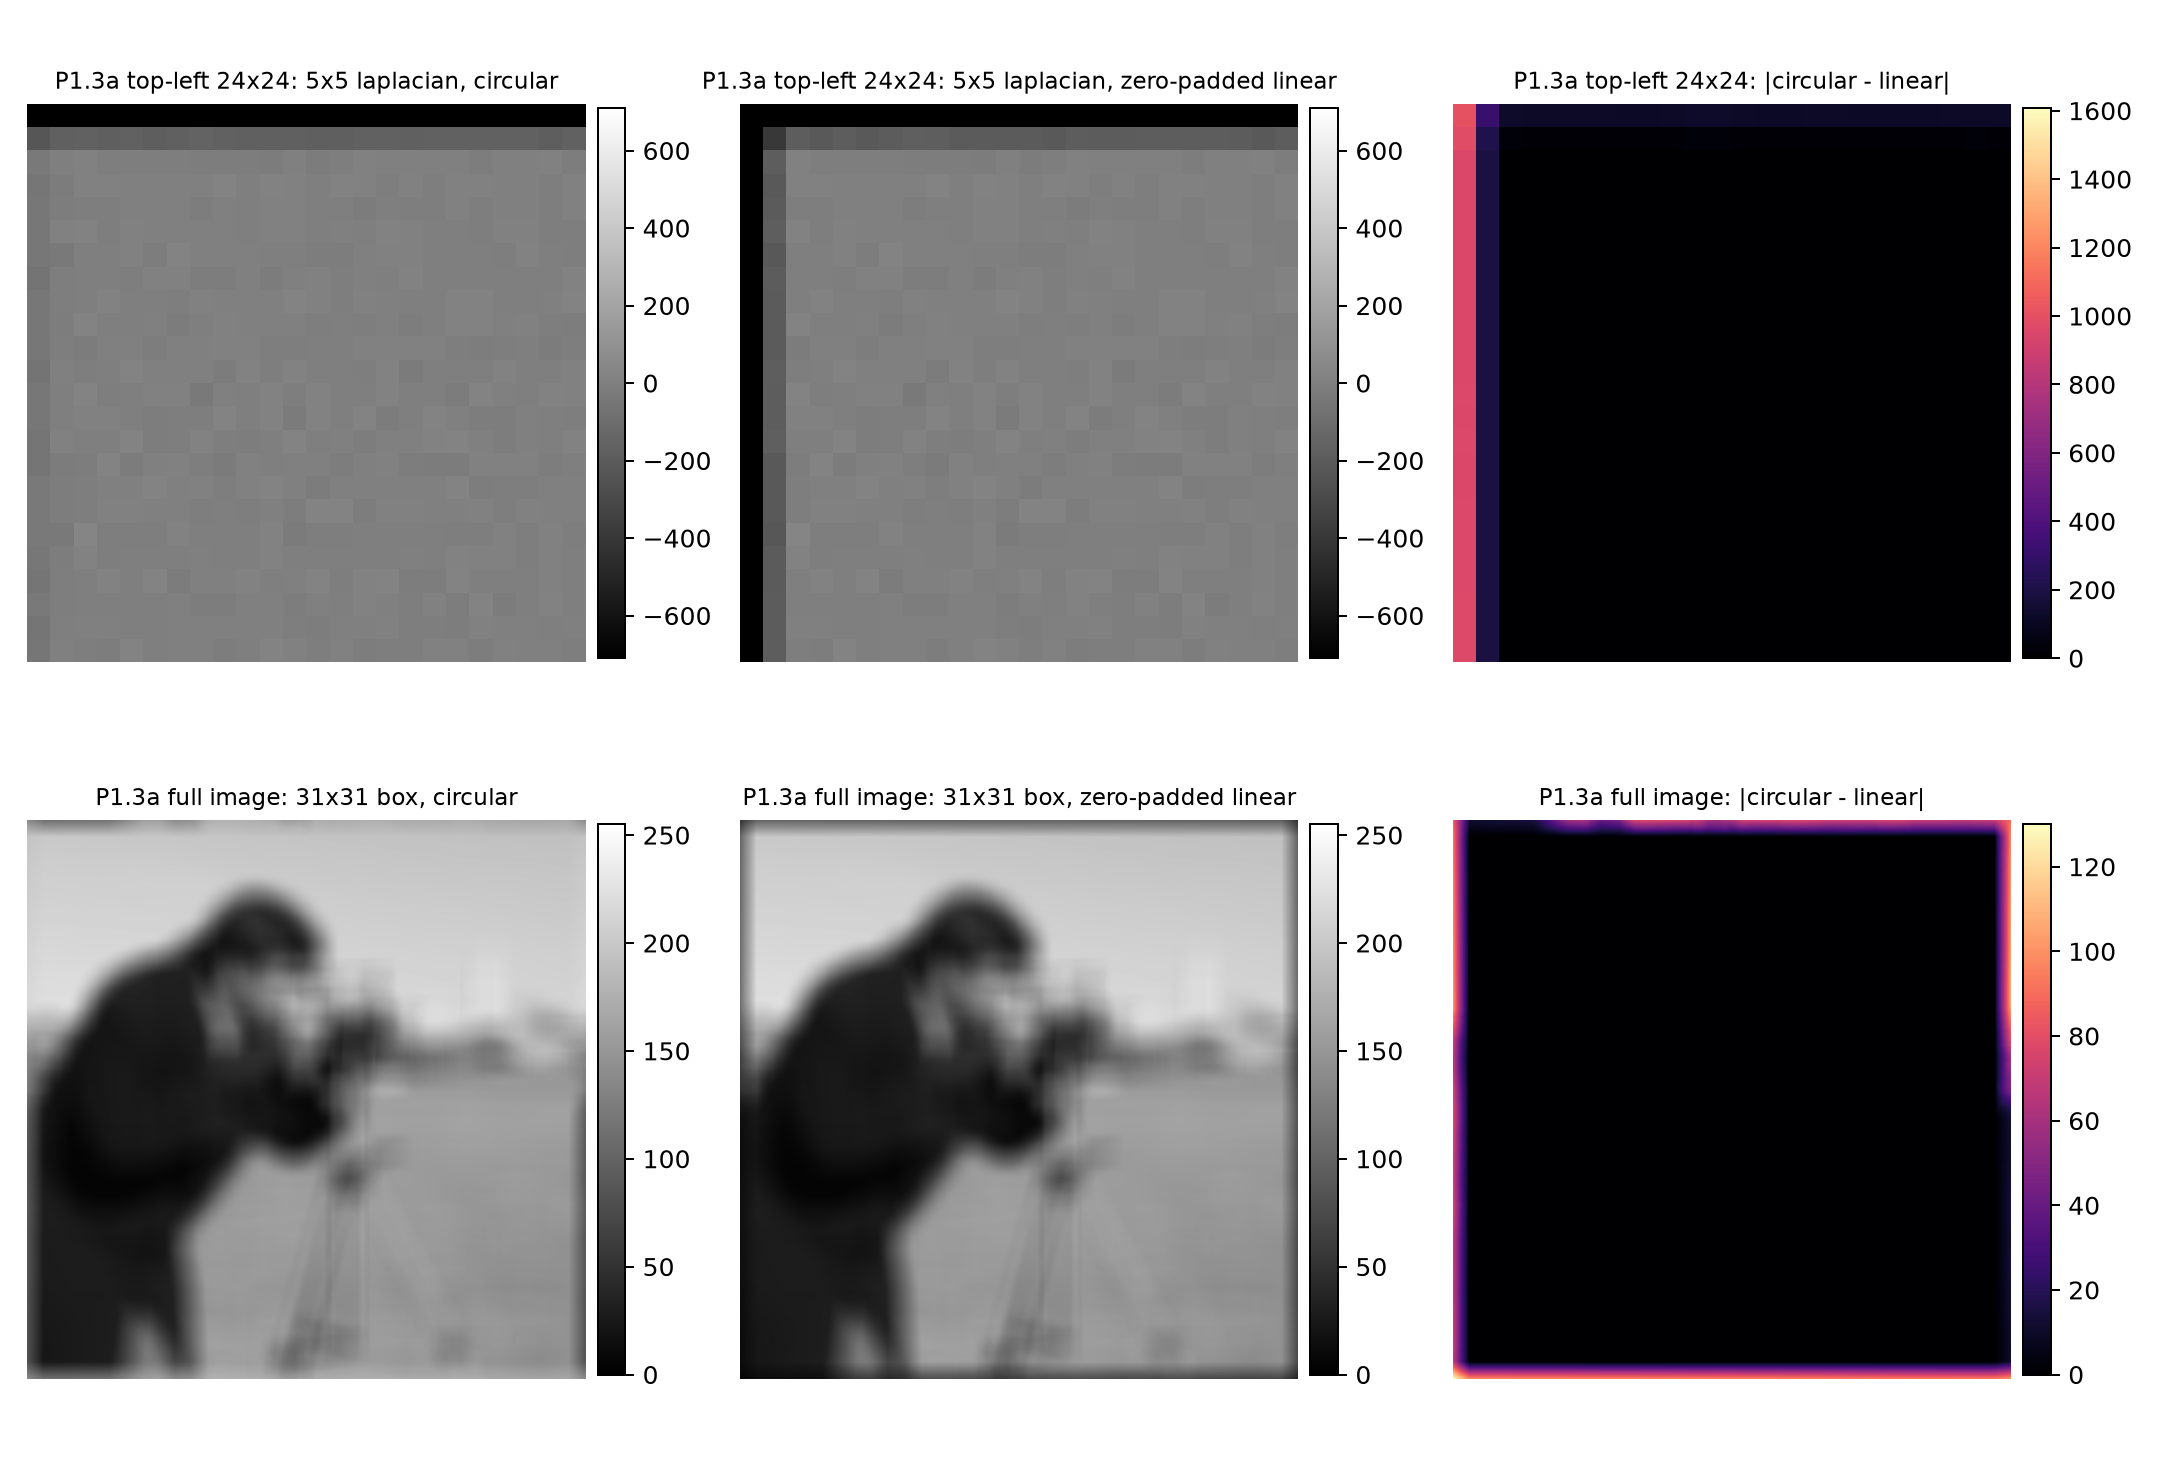
\includegraphics[width=0.9\linewidth]{problem_1/wraparound.png}
\caption{Top: $24\times24$ top-left corner for the $5\times5$ Laplacian. Bottom:
the same comparison with a $31\times31$ box blur over the whole image.}
\label{fig:wrap}
\end{figure}

\paragraph{(b) Cost of padding.} Padding both arrays from $N^2$ to $P^2$ multiplies
every array in the pipeline by $(P/N)^2$: 1.0157 for the minimal $P=516$ and 4 for
the $P=2N$ rule used in Problem 2. The tracemalloc peaks in Table~\ref{tab:pad}
follow this exactly (16.00 MiB to 16.25 MiB to 64.00 MiB). The FFT cost
$O(P^2\log P)$ grows by $(P/N)^2\log P/\log N$: 1.017 for 516 and 4.44 for 1024.
The measured times follow the model only roughly, because FFT speed depends on the
prime factors of $P$. $516=2^2\cdot3\cdot43$ contains the prime 43 and takes
1.40$\times$ the time of $N=512$, while 525 and 540 have only small factors and run
faster than 512 itself. Why the power of two is slower here was not investigated;
strided column passes hitting the same cache sets is one possible reason.
\code{scipy.signal.fftconvolve} handles this trade-off internally. It pads each axis
to the full linear size and then up to \code{next\_fast\_len}$(516,\text{real}=\text{True})=540$,
a 5-smooth size, spending 11\,\% more memory than the minimum to avoid the slow
prime factor, and uses real-input FFTs (\code{rfftn}) that only compute half the
spectrum, which is the redundancy from 1.1a. It took 3.07 ms against 9.40 ms for
the minimal-size complex pipeline.

\begin{table}[H]
\centering
\begin{tabular}{lrlrrrrrr}
\toprule
Grid & $P$ & factors & $(P/N)^2$ & ops ratio & time (ms) & time ratio & MiB & mem.\ ratio\\
\midrule
$N$ (circular) & 512 & $2^9$ & 1.0000 & 1.0000 & 6.723 & 1.000 & 16.00 & 1.000\\
$N+M-1$ & 516 & $2^2\cdot3\cdot43$ & 1.0157 & 1.0170 & 9.400 & 1.398 & 16.25 & 1.016\\
next fast, real & 540 & $2^2\cdot3^3\cdot5$ & 1.1124 & 1.1219 & 6.084 & 0.905 & 17.80 & 1.112\\
next fast, complex & 525 & $3\cdot5^2\cdot7$ & 1.0514 & 1.0557 & 5.581 & 0.830 & 16.83 & 1.051\\
$2N$ (Problem 2) & 1024 & $2^{10}$ & 4.0000 & 4.4444 & 31.140 & 4.632 & 64.00 & 4.000\\
\bottomrule
\end{tabular}
\caption{Cost of the padded pipeline (\code{fft2} of image and kernel, product,
\code{ifft2}), $N=512$, $M=5$. ``ops ratio'' is $P^2\log P/(N^2\log N)$; MiB is the
tracemalloc peak. Times are medians of 41 interleaved runs.}
\label{tab:pad}
\end{table}

\paragraph{Conclusion.} The matrix DFT agrees with \code{numpy.fft} to float64
round-off, and the symmetry, shift and convolution properties hold to the same
precision. Phase carries where things are and magnitude carries how much of each
frequency there is, and the Rayleigh-based prediction for the noise-magnitude
reconstruction was confirmed to within 0.5\,\%. Exact linear convolution needs a
grid of $N+M-1$; in practice the size is rounded up to a fast FFT length.
